\documentclass[UTF8]{ctexart}

%固定图片位置
\usepackage{float}

%插入超链接
\usepackage{url}

\usepackage{tikz,mathpazo}
\usetikzlibrary{shapes.geometric, arrows}
\usetikzlibrary{calc}


\usepackage{listings}
%插入代码的配置
\definecolor{CPPLight}  {HTML} {686868}
\definecolor{CPPSteel}  {HTML} {888888}
\definecolor{CPPDark}   {HTML} {262626}
\definecolor{CPPBlue}   {HTML} {4172A3}
\definecolor{CPPGreen}  {HTML} {487818}
\definecolor{CPPBrown}  {HTML} {A07040}
\definecolor{CPPRed}    {HTML} {AD4D3A}
\definecolor{CPPViolet} {HTML} {7040A0}
\definecolor{CPPGray}  {HTML} {B8B8B8}
\lstset{
	language=Python,                                     % 设置语言
    columns=fixed,    
    breaklines = true,   
    basicstyle=\small ,
    numbers=left,                                        % 在左侧显示行号
    %frame=none,                                          % 不显示背景边框
    backgroundcolor=\color[RGB]{245,245,244},            % 设定背景颜色
    keywordstyle=\color[RGB]{40,40,255},                 % 设定关键字颜色
    numberstyle=\tiny\color{darkgray},           % 设定行号格式
    %commentstyle=\it\color[RGB]{0,96,96},                % 设置代码注释的格式
    stringstyle=\rmfamily\slshape\color[RGB]{128,0,0},   % 设置字符串格式
    showstringspaces=false,                              % 不显示字符串中的空格                           
    %morekeywords={True,alignas,continute,friend,register,true,alignof,decltype,goto,
    %reinterpret_cast,try,asm,defult,if,return,typedef,auto,delete,inline,short,
    %typeid,bool,do,int,signed,typename,break,double,long,sizeof,union,case,
    %dynamic_cast,mutable,static,unsigned,catch,else,namespace,static_assert,using,
    %char,enum,new,static_cast,virtual,char16_t,char32_t,explict,noexcept,struct,
    %void,export,nullptr,switch,volatile,class,extern,operator,template,wchar_t,
    %const,false,private,this,while,constexpr,float,protected,thread_local,
    %const_cast,for,public,throw,std,rand},
    emph={access,and,break,class,continue,def,del,elif ,else,%
	except,exec,finally,for,from,global,if,import,in,i s,%
	lambda,not,or,pass,print,raise,return,try,while},
    emphstyle=\color{CPPViolet}, 
    emph={[2]True, False, None, self},
	emphstyle=[2]\color{green},
	emph={[3]from, import, as},
	emphstyle=[3]\color{blue},
	upquote=true,
	morecomment=[s]{"""}{"""},
	commentstyle=\color{orange}\slshape,
	emph={[4]1, 2, 3, 4, 5, 6, 7, 8, 9, 0},
	emphstyle=[4]\color{red},
	emph={[5]numpy, np, plt},
	emphstyle=[5]\color{red},
	literate=*{:}{{\textcolor{blue}:}}{1}%
	{=}{{\textcolor{blue}=}}{1}%
	{-}{{\textcolor{blue}-}}{1}%
	{+}{{\textcolor{blue}+}}{1}%
	{*}{{\textcolor{blue}*}}{1}%
	{!}{{\textcolor{blue}!}}{1}%
	{(}{{\textcolor{blue}(}}{1}%
	{)}{{\textcolor{blue})}}{1}%
	{[}{{\textcolor{blue}[}}{1}%
	{]}{{\textcolor{blue}]}}{1}%
	{<}{{\textcolor{blue}<}}{1}%
	{>}{{\textcolor{blue}>}}{1},%
	framexleftmargin=0.1mm, framextopmargin=0.1mm, frame=shadowbox, rulesepcolor=\color{black},
}



\usepackage{geometry}
\geometry{left=2cm, right=2cm, top=1.2cm, bottom=1.2cm}

%得到引用的标题内容
\usepackage{nameref} 

%添加首行缩进,两个字符
\usepackage{indentfirst}
\setlength{\parindent}{2em}

%多行公式一个编号
\usepackage{amsmath}

%文献引用,标准类型为plain
%\usepackage[hyperref=true,backend=biber,sorting=none,backref=true]{biblatex}
%\addbibresource{ref.bib}
\bibliographystyle{plain}
\usepackage{cite}

\pagestyle{plain}

%跨页表格
\usepackage{multirow}
\usepackage{longtable,booktabs}
\usepackage{supertabular}
\usepackage{makecell}

%调整itemize等的间距
\usepackage{enumitem}


\usepackage{graphicx}
\usepackage{subfigure}

%超链接
\usepackage[linkcolor=yellow,citecolor=red,backref=page,hyperfootnotes=true]{hyperref}
\hypersetup{
bookmarks=true,
colorlinks=true,
linkcolor=black
}
\usepackage{tabularx} %This package must be placed after package {hyperref}, otherwise footnote marks are NOT treated as hyperlinks.


%引入了一些改进的数学环境,如align
\usepackage{amsmath}

\title{数据结构:The Art of Compression}
\author{姓名:鲁国锐 \protect\newline
\and 学号:17020021031 \\
\and 专业:电子信息科学与技术}
\date{2019.4.18    Thursday}

\begin{document}
	\maketitle
	\renewcommand{\contentsname}{Contents}
	\tableofcontents
	\newpage
	
	\hypersetup{
	bookmarks=true,
	colorlinks=true,
	linkcolor=red,
	urlcolor=blue
	}
	\section{问题分析}
	\subsection{题目描述}
	\indent 本次任务要求对图像进行有针对性的模糊化,即颜色多样性越低的地方模糊程度越大,颜色多样性越高的地方模糊程度越低。具体而言,我们的任务就是将给定的代码补全,使其能够正常运行并输出正确的结果。

	\subsection{问题分析}
	\indent 根据题目及代码,我们需要解决的问题有:
	\begin{enumerate}[leftmargin=50pt]
	\item 根据$stats.h$文件写出$stats.cpp$文件(见\ref{stats}节);
	\item 根据$twoDTree.h$文件写出$twoDTree.cpp$文件(见\ref{twoDTree}节);
	\end{enumerate}
	

	
	\section{解决方案}
		\subsection{$stats$}\label{stats}
		\indent $stats$这个类是专门用来辅助构建二叉树的。更具体的说,是为了让我们能够在常数时间内算出给定范围的矩形内所有元素的和、平方和、平均值以及多样性分数($variability\ score$)。
		
			\subsubsection{构造函数}
			\indent 这里需要我们初始化的成员变量是六个$vector$,其中的第$y$行第$x$列的元素代表的是对应的$PNG$通道中以$(0,0)$为左上角、以$(x, y)$为右下角的矩形中所有元素之和或平方和。为减少计算量,这里我们采取“\textbf{动态规划}”的思想,可以得到状态转移方程:
			\begin{align}
			dp[i][j] = dp[i-1][j] + dp[i][j-1] - dp[i-1][j-1] + im.getPixel(j, i) \label{construction}
			\end{align}
			
			\indent 由于$dp[i-1][j-1]$是$dp[i-1][j]$和$dp[i][j-1]$都包含的部分,相加的时候被算了两次,所以需要减掉一个。\textbf{另外值得注意的一点是,整个工程中涉及到的所有有关坐标的变量或函数,其第一个值代表的是横坐标,即横向的偏移量,对应过来相当于是列下标;而第二个值是纵坐标,即纵向的偏移量,对应过来是行下标。所以这里我们在调用$getPixel$函数是要把$i$、$j$交换位置。}
			
			\indent 当然,方程\ref{construction}在第一行和第一列上是不成立的,在程序中会导致越界,所以这里我们先单独把第一行和第一列的值填上,再从$(1, 1)$开始执行\ref{construction}式。
				
			\subsubsection{$getSum$和$getSumsq$函数}
			\indent 有了那六个$vector$作为辅助,这两个函数实现起来就会轻松许多。这里我们直接给出公式:	
			\begin{align}
			&given\ ul(x1, y1),\ lr(x2, y2): \\			
			&sum(ul, lr) = dp[y2][x2] - dp[y1-1][x2] - dp[y2][x1-1] + dp[y1-1][x1-1] \label{sum}
			\end{align}
		    
		    \indent 同样,\ref{sum}式在$ul$在第一行或第一列上时是不成立的,以在第一行(不包括原点)上为例:
		    \begin{align}
		    sum(ul, lr) = dp[y2][x2] - dp[y2][x1-1] \label{sum_first_row}
		    \end{align}

            \indent 参照\ref{construction}式和\ref{sum_first_row}式我们能得出$ul$在第一列或原点上的表达式。
            
            \indent $getSumsq$原理同$getSum$。
            
            \subsubsection{$getScore$函数}
            \indent 根据文档中给出的等式:
            \begin{align}
            \sum(x - \bar{x})^{2} = \sum x^2 - \frac{(\sum x)^2}{|R|} \label{score}
            \end{align} 
            
            \indent 再结合$getSum$和$getSumsp$函数,我们可以在$O(1)$时间内算出其多样性分数。
            \subsubsection{$getArea$和$getAvg$函数}  
            \indent 这里的$getArea$函数其实是为$getAvg$服务的。我们先用$getSum$求出对应通道中像素值的和,再将其除以$getArea$返回的数量即得平均值。平均值仍然分$r$、$g$、$b$三个通道,用一个$RGBAPixel$存放。\textbf{注意这里的$RGBAPixel$类中还定义了一个透明度通道,但这里我们不会涉及到它,直接遵循默认设定将其置为1即可}。      		    
		\subsection{$twoDTree$}\label{twoDTree}
		
		\indent 这一块是整个算法最核心的部分。其中构造函数和剪枝函数是最关键的两个部分,我们重点来看一看这两个函数的设计。
		
		\subsubsection{构造函数}
		\indent 这里并没有采用$K-D$树中“深度为偶数垂直分割,深度为奇数水平分割”的构造策略,而是对当前矩形的长宽进行比较,若长大于宽,水平分隔;反之则垂直分割。这里我还专门在$Node$里面加了一个成员变量$flag$来记录对当前矩形是做的垂直分割还是水平分割。现在想想其实这个变量完全没必要,因为$Node$中本身就有$upLeft$和$lowRight$这两个对组,我们只需要简单算一下当前矩形的长和宽就可以知道是做的什么分割了。
		
		\indent 在做分割时,我们用一个对组来记录坐标,沿着一条边走,计算被过这个点的垂线所分成的两个小矩形的多样性分数\textbf{之和}。以垂直分割为例,设左上角的坐标为$(x1, y1)$,右下角的坐标为$(x2, y2)$,我们令一个点$i$的初始坐标为$(x1, y2)$,让其沿$y = y2$这条直线向右移动,同时令另一个点$j$的初始坐标为$(x1+1, y1)$,沿着$y = y1$向右移动。这样在移动的过程中$i$始终是左边矩形的右下角,而$j$始终是右边矩形的左上角。在此过程中我们不断计算两个矩形的多样性分数。\textbf{而考虑到两个矩形的多样性分数可能不会同时达到最小,所以这里我们取令二者之和最小的分割方式}。然后再递归地进行下去,直至当前矩形的左上角坐标等于右下角,即矩形中只有一个元素时,停止递归,并返回当前节点的指针。
		
		\indent 除了分割外我们还需要调用$stats$类,来帮我们计算出该矩形范围内$RGB$通道的平均值,记录在$RGBAPixel$类型的成员变量$avg$中,另外我还额外给节点类增加了一个变量$split\_value$,用来记录分割的位置。
		
		\subsubsection{剪枝函数}
		\indent 这里我们再明确一下剪枝的要求:\textcolor[rgb]{0.8,0.1,0.1}{给定两个值$percent$和$tolerance$,我们对某一棵子树计算其根节点与每一个叶节点$avg$之差的平方(注意这里要把三个通道的值都加起来),如果计算出来的值大于$tolerance$且这样的叶节点数量占总数的比例大于$percent$,我们就要给这个子树剪枝,即只保留根节点}。
		
		\indent 但对每一个节点都执行一次遍历子树的操作计算成本太高,我们希望能够对每个节点只遍历一次。所以这里我们用$vector$来作为函数的返回值。当碰到叶节点时,我们将叶节点放入一个向量中返回;而对于其它节点,先进行递归得到左右子树的叶节点,将两个向量合并之后再开始判断是否需要剪枝,最后返回合并后的向量即可。
		
		\subsubsection{$render$函数、$copy$函数和$clear$函数}
		\indent 在$render$函数中,我们要实例化一个$PNG$对象,然后根据每一个像素的坐标	在构建好的二叉树中找到相应的节点,把该节点的$avg$赋值过来即可。
		
		\indent $copy$函数和$clear$函数比较简单,在此不做赘述。	
	
	\section{算法设计}
	见图\ref{buildTree}、图\ref{main}


\begin{figure}[H]
	\centering 
	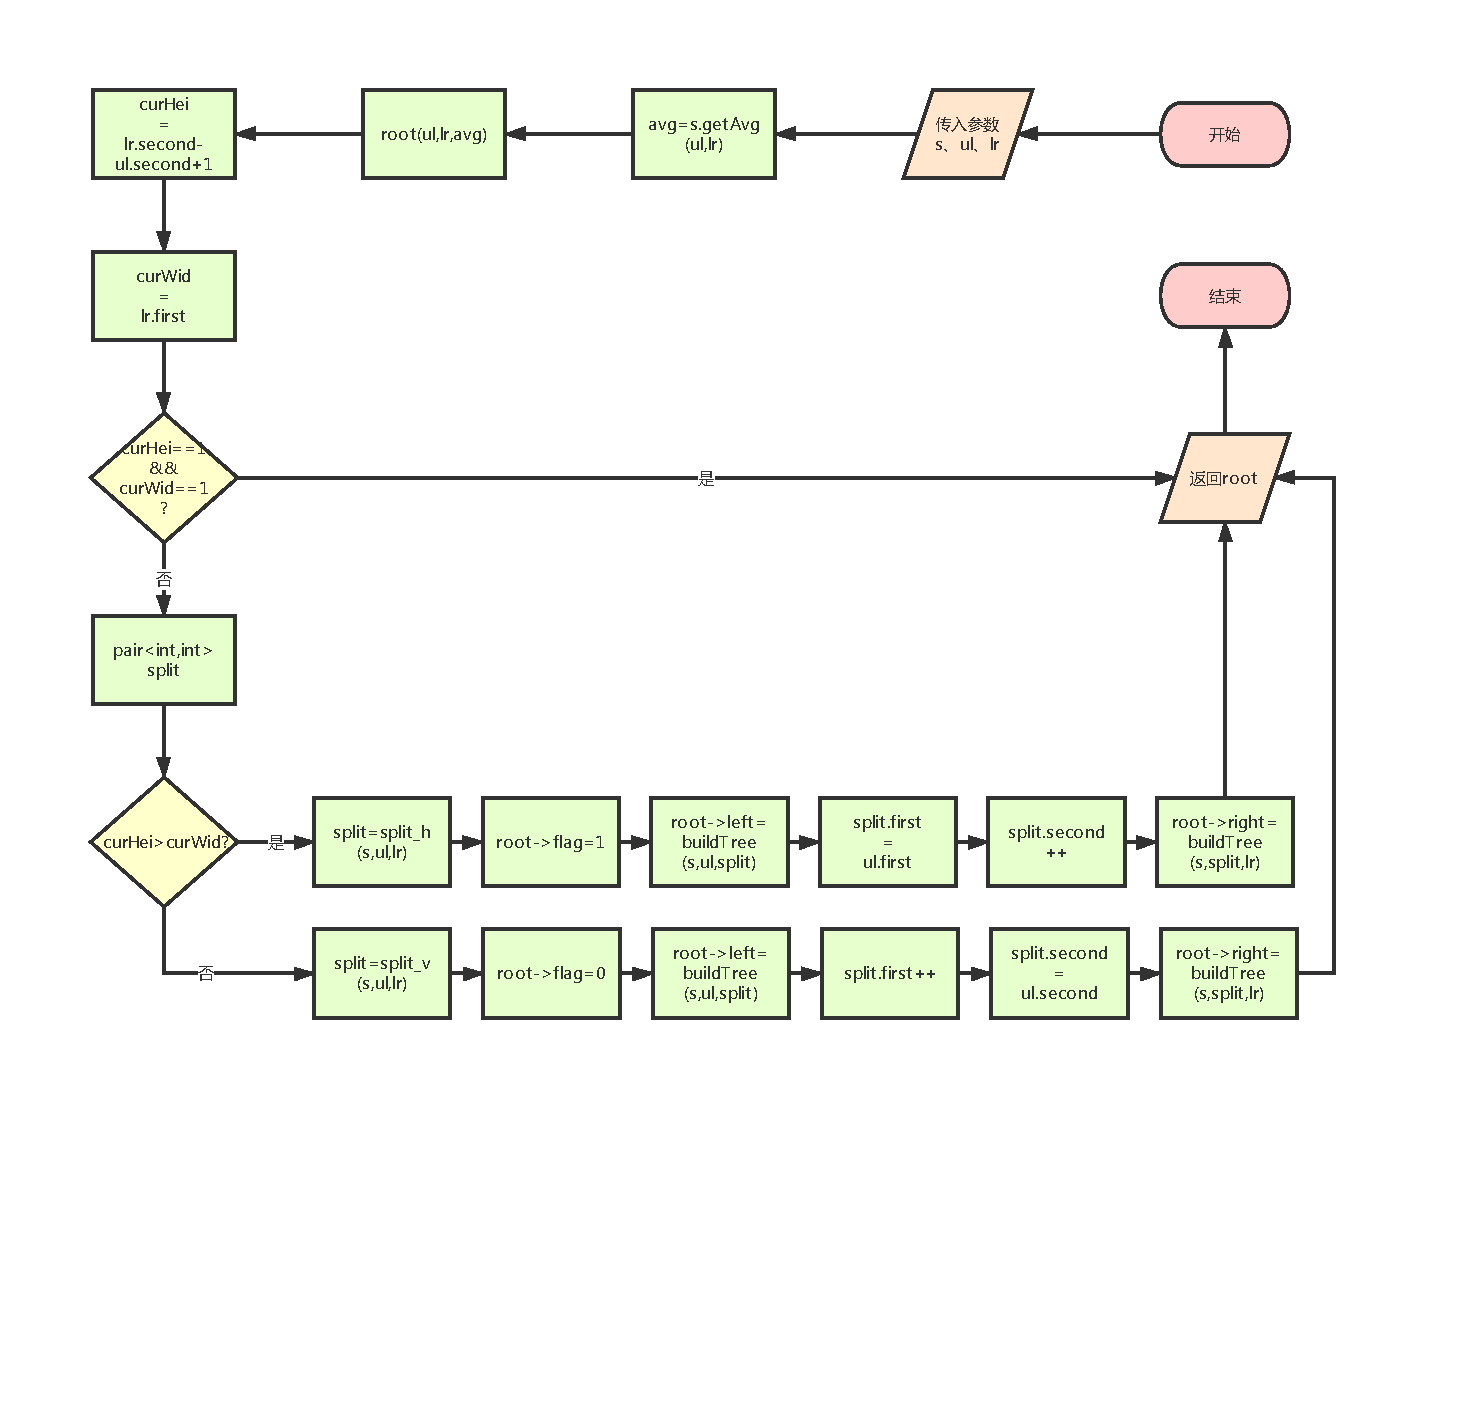
\includegraphics[width=20cm, height=19cm]{buildTree.pdf} 
	\caption{$buildTree$函数流程图} 
	\label{buildTree}
\end{figure}



\begin{figure}[H]
	\centering 
	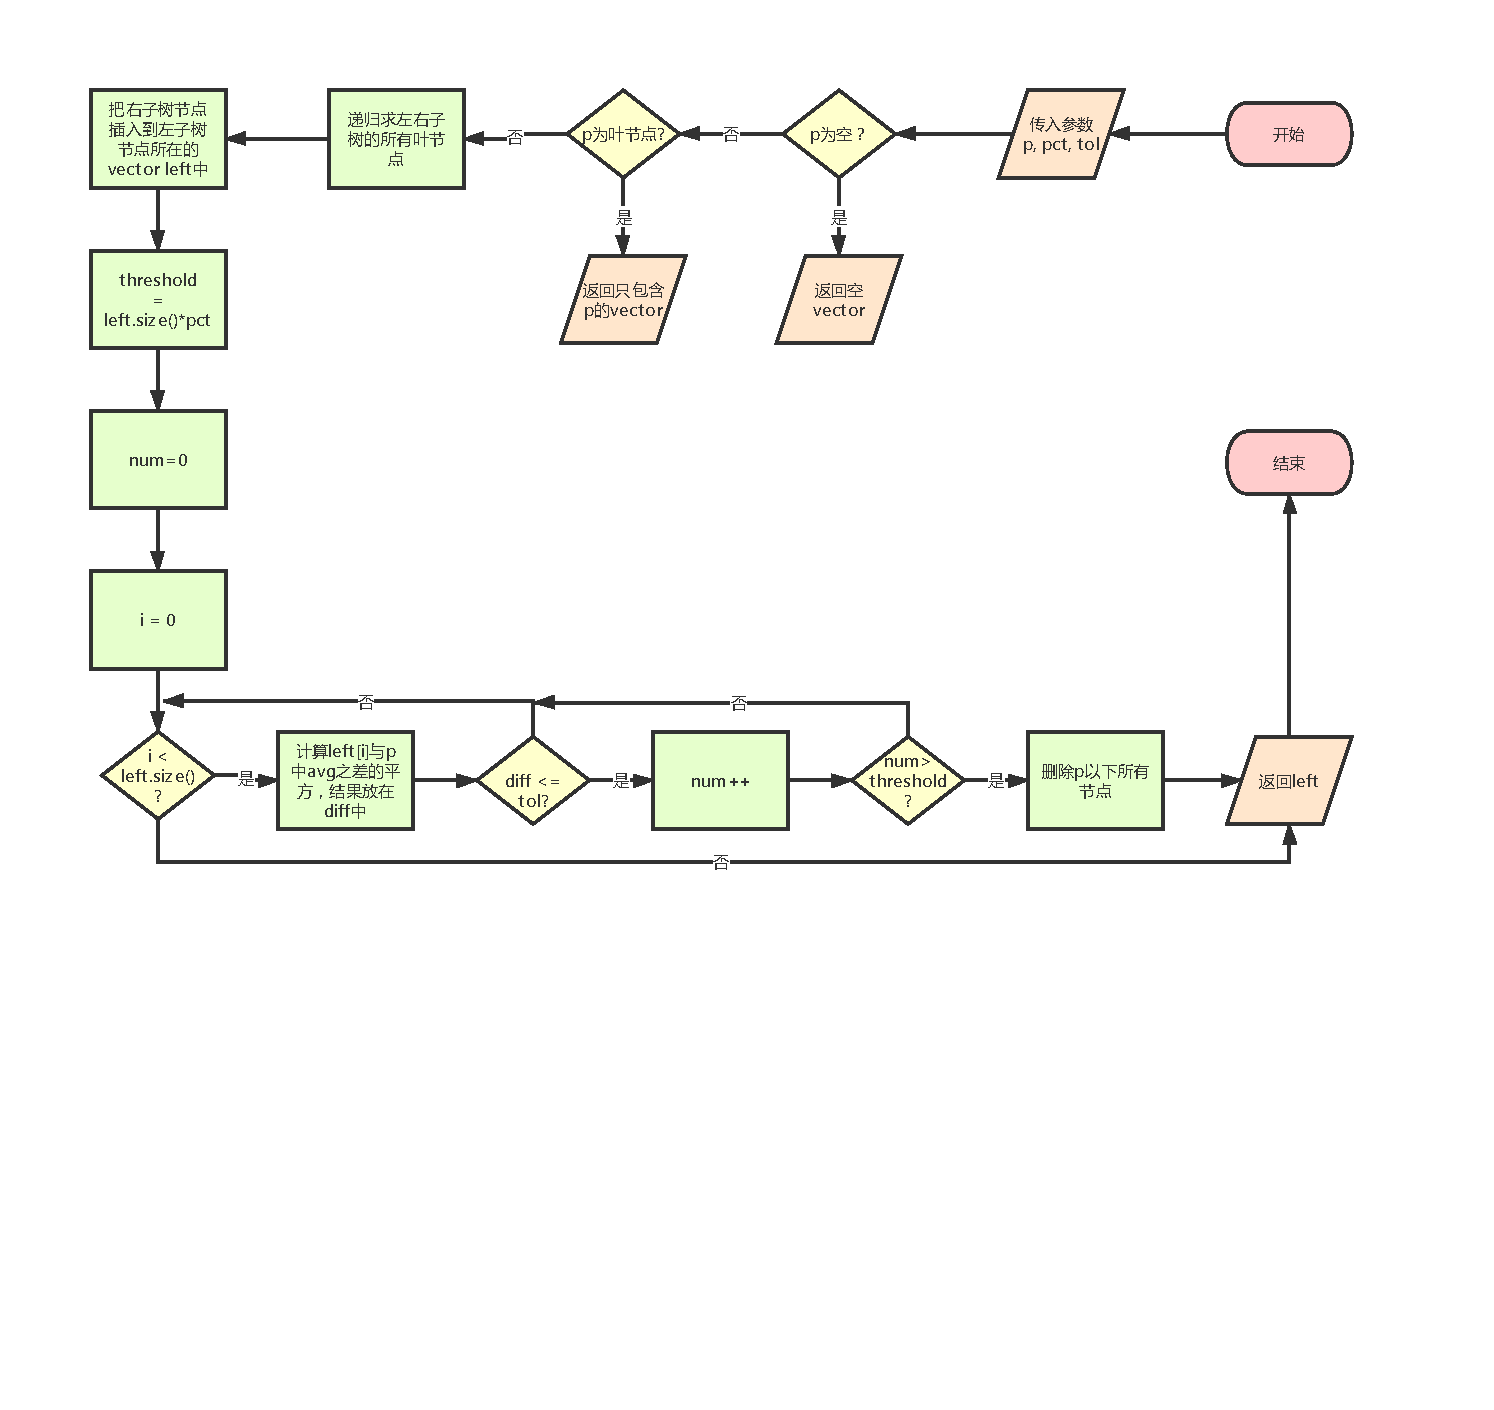
\includegraphics[width=20cm, height=23cm]{prune.pdf} 
	\caption{$prune$函数流程图} 
	\label{main}
\end{figure}
\newpage



	\section{编程实现\protect \footnotemark[1]}
	\footnotetext[1]{完整的代码:\url{https://github.com/chenfeng123456/CourseInOUC/tree/master/algorithm/pa3_sourcecode}}

	\begin{lstlisting}[language=C++,caption={stats.cpp},label={stats.cpp}]
#include "stats.h"
#include <iostream>
#include <cmath>

stats::stats(PNG &im)
{
    for (int i=0; i < im.height(); i++)
    {
        sumRed.push_back(vector<long>(im.width()));
        sumsqRed.push_back(vector<long>(im.width()));

        sumGreen.push_back(vector<long>(im.width()));
        sumsqGreen.push_back(vector<long>(im.width()));

        sumBlue.push_back(vector<long>(im.width()));
        sumsqBlue.push_back(vector<long>(im.width()));
    }
    
    sumRed[0][0] = im.getPixel(0, 0)->r;
    sumsqRed[0][0] = pow(im.getPixel(0, 0)->r, 2);
    
    sumGreen[0][0] = im.getPixel(0, 0)->g;
    sumsqGreen[0][0] = pow(im.getPixel(0, 0)->g, 2);
    
    sumBlue[0][0] = im.getPixel(0, 0)->b;
    sumsqBlue[0][0] = pow(im.getPixel(0, 0)->b, 2);

    for (int i=1; i < im.height(); i++)
    {
        sumRed[i][0] = im.getPixel(0, i)->r + sumRed[i-1][0];
        sumsqRed[i][0] = pow(im.getPixel(0, i)->r, 2) + sumsqRed[i-1][0];

        sumGreen[i][0] = im.getPixel(0, i)->g + sumGreen[i-1][0];
        sumsqGreen[i][0] = pow(im.getPixel(0, i)->g, 2) + sumsqGreen[i-1][0];

        sumBlue[i][0] = im.getPixel(0, i)->b + sumBlue[i-1][0];
        sumsqBlue[i][0] = pow(im.getPixel(0, i)->b, 2) + sumsqBlue[i-1][0];
    }
    for (int i=1; i < im.width(); i++)
    {
        sumRed[0][i] = im.getPixel(i, 0)->r + sumRed[0][i-1];
        sumsqRed[0][i] = pow(im.getPixel(i, 0)->r, 2) + sumsqRed[0][i-1];

        sumGreen[0][i] = im.getPixel(i, 0)->g + sumGreen[0][i-1];
        sumsqGreen[0][i] = pow(im.getPixel(i, 0)->g, 2) + sumsqGreen[0][i-1];

        sumBlue[0][i] = im.getPixel(i, 0)->b +sumBlue[0][i-1];
        sumsqBlue[0][i] = pow(im.getPixel(i, 0)->b, 2) + sumsqBlue[0][i-1];
    }
    for (int i=1; i < im.height(); i++)
    {
        for (int j=1; j < im.width(); j++)
        {
            sumRed[i][j] = sumRed[i-1][j] + sumRed[i][j-1] - sumRed[i-1][j-1] + im.getPixel(j, i)->r;
            sumsqRed[i][j] = sumsqRed[i-1][j] + sumsqRed[i][j-1] -sumsqRed[i-1][j-1] + pow(im.getPixel(j, i)->r, 2);

            sumGreen[i][j] = sumGreen[i-1][j] + sumGreen[i][j-1] - sumGreen[i-1][j-1] + im.getPixel(j, i)->g;
            sumsqGreen[i][j] = sumsqGreen[i-1][j] + sumsqGreen[i][j-1] - sumsqGreen[i-1][j-1] + pow(im.getPixel(j, i)->g, 2);

            sumBlue[i][j] = sumBlue[i-1][j] + sumBlue[i][j-1] - sumBlue[i-1][j-1] + im.getPixel(j, i)->b;
            sumsqBlue[i][j] = sumsqBlue[i-1][j] + sumsqBlue[i][j-1] - sumsqBlue[i-1][j-1] + pow(im.getPixel(j, i)->b, 2);
        }
    }


    /*
    cout << "image.width() = " << im.width() << endl;
    cout << "image.height() = " << im.height() << endl;
    cout << "sumRed[0].size() = " << sumRed[0].size() << endl;
    cout << "sumRed.size() = " << sumRed.size() << endl;
    */

    cout << "im:" << endl;
    for (int i = 0; i < 5; i++)
    {
        for (int j = 0; j < 5; j++)
            cout << (long)im.getPixel(j, i)->b << "  ";
        cout << endl;
    }
    cout << endl;
    cout << "sumBlue:" << endl;
    for (int i=0; i < 5; i++)
    {
        for (int j=0; j < 5; j++)
            cout << sumBlue[i][j] << "  ";
        cout << endl;
    }
    cout << endl;
    cout << "sumsqBlue:" << endl;
    for (int i=0; i < 5; i++)
    {
        for (int j=0; j < 5; j++)
            cout << sumsqBlue[i][j] << "  ";
        cout << endl;
    }
    cout << endl;
    
    pair<int, int> ul(2, 2);
    pair<int, int> lr(2, 2);
    cout << "getSum((2,2), (2,2)):  " << getSum('b', ul, lr) << endl;
    cout << "getSum((2,2), (2,2)):  " << getSumSq('b', ul, lr) << endl;
    cout << "getavg((2,2), (2,2)):  " << (int)getAvg(ul, lr).b << endl << endl;

}

long stats::getSum(char channel, pair<int, int> ul, pair<int, int> lr)
{
    if (channel == 'r')
    {
		long rec1 = (ul.second == 0 ? 0 : sumRed[ul.second-1][lr.first]);
        long rec2 = (ul.first == 0 ? 0 : sumRed[lr.second][ul.first-1]);
        long rec3 = ((ul.second == 0 || ul.first == 0) ? 0 : sumRed[ul.second-1][ul.first-1]);
        return sumRed[lr.second][lr.first] - rec1 - rec2 + rec3;   
	}
    else if (channel == 'g')
    {
		long rec1 = (ul.second == 0 ? 0 : sumGreen[ul.second-1][lr.first]);
        long rec2 = (ul.first == 0 ? 0 : sumGreen[lr.second][ul.first-1]);
        long rec3 = ((ul.second == 0 || ul.first == 0) ? 0 : sumGreen[ul.second-1][ul.first-1]);
        return sumGreen[lr.second][lr.first] - rec1 - rec2 + rec3;
	}
    else if (channel == 'b')
    {
		long rec1 = (ul.second == 0 ? 0 : sumBlue[ul.second-1][lr.first]);
        long rec2 = (ul.first == 0 ? 0 : sumBlue[lr.second][ul.first-1]);
        long rec3 = ((ul.second == 0 || ul.first == 0) ? 0 : sumBlue[ul.second-1][ul.first-1]);
        return sumBlue[lr.second][lr.first] - rec1 - rec2 + rec3;
	}
    else
    {
        cerr << "Invalid channel!" << endl;
        return -1;
    }
}

long stats::getSumSq(char channel, pair<int, int> ul, pair<int, int> lr)                                                                                    
{                                                                                                                                                         
    if (channel == 'r')                                                                                                                                   
    {
        long rec1 = (ul.second == 0 ? 0 : sumsqRed[ul.second-1][lr.first]);
        long rec2 = (ul.first == 0 ? 0 : sumsqRed[lr.second][ul.first-1]);
        long rec3 = ((ul.second == 0 || ul.first == 0) ? 0 : sumsqRed[ul.second-1][ul.first-1]);
        return sumsqRed[lr.second][lr.first] - rec1 - rec2 + rec3;             
    }
    else if (channel == 'g')                                                                                                                              
    {
        long rec1 = (ul.second == 0 ? 0 : sumsqGreen[ul.second-1][lr.first]);
        long rec2 = (ul.first == 0 ? 0 : sumsqGreen[lr.second][ul.first-1]);
        long rec3 = ((ul.second == 0 || ul.first == 0) ? 0 : sumsqGreen[ul.second-1][ul.first-1]);
        return sumsqGreen[lr.second][lr.first] - rec1 - rec2 + rec3;        
    }
    else if (channel == 'b')                                                                                                                              
    {
        long rec1 = (ul.second == 0 ? 0 : sumsqBlue[ul.second-1][lr.first]);
        long rec2 = (ul.first == 0 ? 0 : sumsqBlue[lr.second][ul.first-1]);
        long rec3 = ((ul.second == 0 || ul.first == 0) ? 0 : sumsqBlue[ul.second-1][ul.first-1]);
        return sumsqBlue[lr.second][lr.first] - rec1 - rec2 + rec3;            
    }
    else                                                                                                                                                  
    {                                                                                                                                                     
        cerr << "Invalid channel!" << endl;                                                                                                               
        return -1;                                                                                                                                        
    }                                                                                                                                                     
}  

long stats::rectArea(pair<int, int> ul, pair<int, int> lr)
{
    return (lr.first - ul.first + 1) * (lr.second - ul.second + 1);
}

long stats::getScore(pair<int, int> ul, pair<int, int> lr)
{
    long R = rectArea(ul, lr);
    long rscore = getSumSq('r', ul, lr) - pow(getSum('r', ul, lr), 2) / R;
    long gscore = getSumSq('g', ul, lr) - pow(getSum('g', ul, lr), 2) / R;
    long bscore = getSumSq('b', ul, lr) - pow(getSum('b', ul, lr), 2) / R;
    return rscore + gscore + bscore;
}

RGBAPixel stats::getAvg(pair<int, int> ul, pair<int, int> lr)
{
    long R = rectArea(ul, lr);
    int avgR = getSum('r', ul, lr) / R;
    int avgG = getSum('g', ul, lr) / R;
    int avgB = getSum('b', ul, lr) / R;
    RGBAPixel avg(avgR, avgG, avgB);
    return avg;
}




	\end{lstlisting}
\begin{lstlisting}[language=C++,caption={twoDTree.cpp},label={twoDTree.cpp}]

/**
 *
 * twoDtree (pa3)
 * slight modification of a Kd tree of dimension 2.
 * twoDtree.cpp
 * This file will be used for grading.
 *
 */

#include <cmath>
#include "twoDtree.h"
#include "cs221util/RGBAPixel.h"

/* given */
twoDtree::Node::Node(pair<int,int> ul, pair<int,int> lr, RGBAPixel a)
	:upLeft(ul),lowRight(lr),avg(a),left(NULL),right(NULL),flag(-1),split_value(-1)
	{}




/* given */
twoDtree::~twoDtree(){
	clear();
}

/* given */
twoDtree::twoDtree(const twoDtree & other) {
	copy(other);
}

/* given */
twoDtree & twoDtree::operator=(const twoDtree & rhs){
	if (this != &rhs) {
		clear();
		copy(rhs);
	}
	return *this;
}

twoDtree::twoDtree(PNG & imIn){ /* your code here */ 
    im = imIn;
    stats s(imIn);
    height = imIn.height();
    width = imIn.width();
    pair<int, int> ul(0, 0);
    pair<int, int> lr(width-1, height-1);
    root = buildTree(s, ul, lr);
}


pair<int, int> split_h(stats &s, pair<int, int> ul, pair<int, int> lr)
{
    // split the rectangle horizontally
    long minScore = 2147483647;
    pair<int, int> res(lr.first, ul.second);
    pair<int, int> i(lr.first, ul.second);
    pair<int, int> j(ul.first, ul.second+1);
    for(; i.second < lr.second; i.second++, j.second++)
    {
        long score = s.getScore(ul, i);
        score += s.getScore(j, lr);
        if (score < minScore)
        {
            minScore = score;
            res.first = i.first;
            res.second = i.second;
        }
    }
    return res;
}

pair<int, int> split_v(stats &s, pair<int, int> ul, pair<int, int> lr)                                                          
{                                                                                                                               
    // split the rectangle vertically                                                                                         
    long minScore = 2147483647;                                                                                                          
    pair<int, int> res(ul.first, lr.second);                                                                                    
    pair<int, int> i(ul.first, lr.second);                                                                                      
    pair<int, int> j(ul.first+1, ul.second);                                                                                    
    for(; i.first < lr.first; i.first++, j.first++)                                                                         
    {                                                                                                                           
        long score = s.getScore(ul, i);                                                                                         
        score += s.getScore(j, lr);                                                                                             
        if (score < minScore)                                                                                                   
        {                                                                                                                       
            minScore = score;                                                                    
            res.first = i.first;
            res.second = i.second;                                                                                              
        }                                                                                                                       
    }                                                                                                                           
    return res;                                                                                                                 
}        


twoDtree::Node * twoDtree::buildTree(stats & s, pair<int,int> ul, pair<int,int> lr) {
	/* your code here */
    RGBAPixel avg = s.getAvg(ul, lr);
    Node *root = new Node(ul, lr, avg);
    int curHei = lr.second - ul.second + 1;
    int curWid = lr.first - ul.first + 1;
    //cout << curHei << ", " << curWid << endl;
  
    if (curHei == 1 && curWid == 1)
    {
        /*
        cout << "(" << ul.first << ", " << ul.second << ")   " << "(" << lr.first << ", " << lr.second << ")" << endl;
        cout << "avg = " << avg << endl;
        cout << "(x,y)=" << *im.getPixel(ul.first, ul.second) << endl;
        if (avg == *im.getPixel(ul.first, ul.second))
            cout << "True" << endl;
        else
        {
            for(int i=0; i < 100; i++)
            {
                for (int j=0; j < 100; j++)
                    cout << "**";
                cout << endl;
            }
        }
                   
            
        cout << endl;
        */
        return root;
    }
    pair<int, int> split;
    if (curHei > curWid)
    {
        split = split_h(s, ul, lr);
        root->flag = 1;
        root->split_value = split.second;
        //cout << "root->split_value = " << root->split_value << endl;
        root->left = buildTree(s, ul, split);
        split.first = ul.first;
        split.second++;
        root->right = buildTree(s, split, lr);
    }
    else
    {
        split = split_v(s, ul, lr);
        root->flag = 0;
        root->split_value = split.first;
        //cout << "root->split_value = " << root->split_value << endl;
        root->left = buildTree(s, ul, split);
        split.first++;
        split.second = ul.second;
        root->right = buildTree(s, split, lr);
    }

    //cout << "(" << ul.first << ", " << ul.second << ")   " << "(" << lr.first << ", " << lr.second << ")" << endl;

    return root;
}


RGBAPixel* twoDtree::render_helper(int const x, int const y, Node *r)
{
    if (r->left == NULL && r->right == NULL)
        return &(r->avg);
    RGBAPixel *p = NULL;
    //cout << "r->avg = " << r->avg << endl;
    //cout << "root->flag = " << r->flag << "   ";
    //cout << "r->split_value = " << r->split_value << "  ";
    //cout << "upLeft = (" << r->upLeft.first << ", " << r->upLeft.second << ")   ";
    //cout << "lowRight=(" << r->lowRight.first << ", " << r->lowRight.second << ")";
    if (r->flag == 1)
    {
        //cout << "  y = " << y << endl;
        if (y <= r->split_value)
            p = render_helper(x, y, r->left);
        else
            p = render_helper(x, y, r->right);

    }
    else
    {
        //cout << "  x = " << x << endl;
        if (x <= r->split_value)
            p = render_helper(x, y, r->left);
        else 
            p = render_helper(x, y, r->right);
    }

    if(!p)
    {
        /*
        if (r->avg == *im.getPixel(x, y))
            cout << "True" << endl;
        else
            cout << "False" << endl;
            */
        return &(r->avg);
    }
    //cout << *p << endl;
    return p;
}


PNG twoDtree::render(){
	/* your code here */
    PNG image(width, height);
    //cout << "width = " << width << "   height = " << height << endl;
    //cout << "image.width = " << image.width() << "   image.height = " << image.height() << endl;
    for (int x=0; x < width; x++)
    {
        for (int y=0; y < height; y++)
        {
            RGBAPixel* p = image.getPixel(x, y);
            cout << "x = " << x << " , y = " << y << endl;
            RGBAPixel* other = render_helper(x, y, root);
            cout << "*****" << endl;
            cout << "(x,y)=" << *im.getPixel(x, y) << endl;
            p->r = other->r; p->g = other->g; p->b = other->b; p->a = other->a;
            cout << "r = " << (int)p->r << "   g = " << (int)p->g << "   b = " << (int)p->b << endl << endl;
            /*
            if ((*p) == (*im.getPixel(x, y)))
                cout << "True" << endl;
            else
            {
                cout << "False" << endl;
            }
            */
        }
    }
    return image;
}

vector<int> twoDtree::prune_helper(Node *p, double const pct, int const tol)
{
    if (!p) 
    {
        vector<int> l;
        return l;
    }
    if (p->left == NULL && p->right == NULL)
    {
        vector<int> l;
        l.push_back(p->avg.r + p->avg.g + p->avg.b);
        return l;
    }


    vector<int> left = prune_helper(p->left, pct, tol);
    vector<int> right = prune_helper(p->right, pct, tol);
    left.insert(left.end(), right.begin(), right.end());

    int threshold = left.size();
    threshold = threshold * pct;
    int num = 0;
    for (int i=0; i < left.size(); i++)
    {
        int avgL = left[i];
        int avgP = p->avg.r + p->avg.g + p->avg.b;
        int diff = pow(avgL-avgP, 2);
        if (diff <= tol)
        {
            num++;
            if (num > threshold)
            {
                cout << (p->left == NULL) << " , " << (p->right == NULL) << endl;
                remove(p);
                break;
            }
        }
    }

    return left;
}


void twoDtree::prune(double pct, int tol){
	/* your code here */
    prune_helper(root, pct, tol);
}

void twoDtree::clear() {
	/* your code here */
    if (root)
    {
        remove(root);
        Node *old = root;
        root = NULL;
        delete old;
    }
}

void twoDtree::remove(Node *root)
{
    if (root->left)
    {
        if (root->left->left || root->left->right)
            remove(root->left);
        Node *old = root->left;
        root->left = NULL;
        delete old;
    }
    
    if (root->right)
    {
        if (root->right->left || root->right->right)
            remove(root->right);
        Node *old = root->right;
        root->right = NULL;
        delete old;
    }

    //cout << root << endl;
}

void twoDtree::copy(const twoDtree & orig){
	/* your code here */
    root = copy_helper(orig.root);
    im = orig.im;
    height = orig.height;
    width = orig.width;

}

twoDtree::Node* twoDtree::copy_helper(const Node *r)
{
    if (!r)
        return NULL;
    
    Node *root = new Node(r->upLeft, r->lowRight, r->avg);
    root->flag = r->flag;
    root->split_value = r->split_value;
    root->left = copy_helper(r->left);
    root->right = copy_helper(r->right);
    root->avg = r->avg;
    //cout << "copy " << r << endl;
    return root;
}

\end{lstlisting}
	\section{结果分析}
	\subsection{结果展示}


\begin{figure}[H]
\centering
\subfigure[原图1]{
\begin{minipage}{0.45\linewidth}
\centering

\includegraphics[width=6cm, height=6cm]{remb.png}
%\caption{原图1}
\end{minipage}%
}%
\subfigure[结果1]{
\begin{minipage}{0.45\linewidth}
\centering
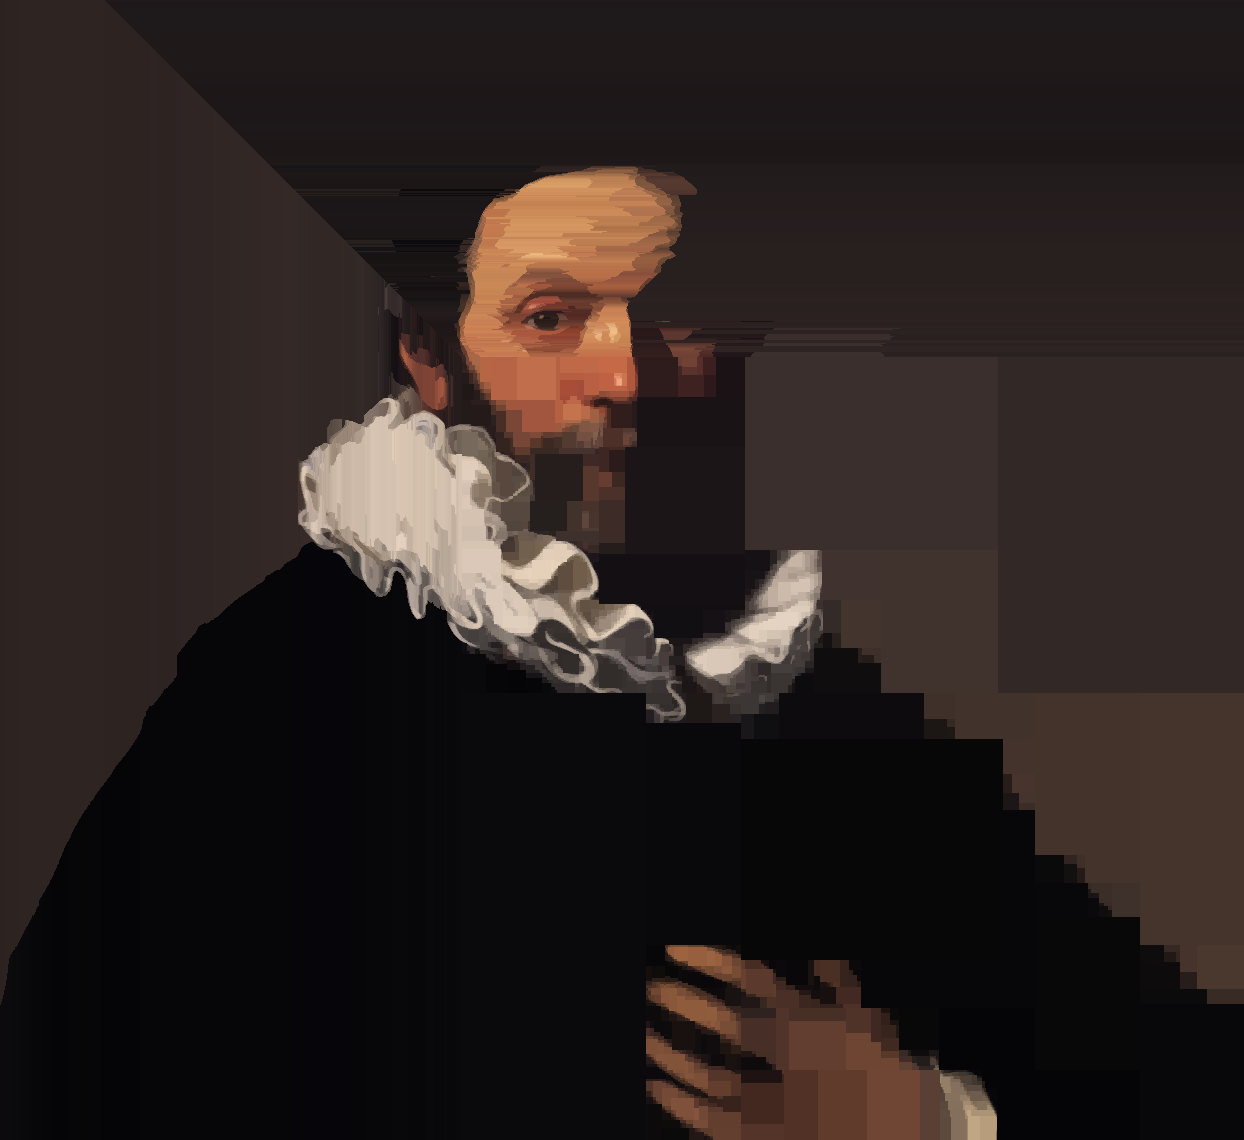
\includegraphics[width=6cm, height=6cm]{prunedremb.png}
%\caption{结果1}
\end{minipage}
}

\subfigure[原图2]{
\begin{minipage}{0.45\linewidth}
\centering
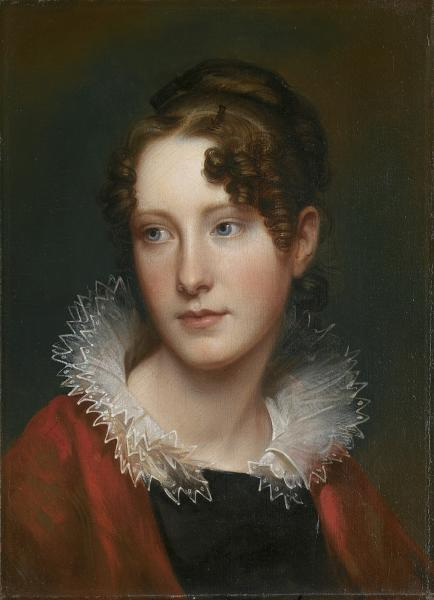
\includegraphics[width=6cm, height=6cm]{rosa.png}
%\caption{原图2}
\end{minipage}%
}%
\subfigure[结果2]{
\begin{minipage}{0.45\linewidth}
\centering
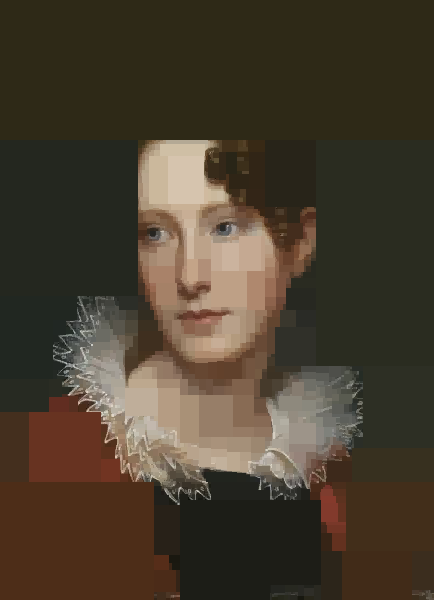
\includegraphics[width=6cm, height=6cm]{prunedrosa.png}
%\caption{结果2}
\end{minipage}
}

\subfigure[原图3]{
\begin{minipage}{0.45\linewidth}
\centering
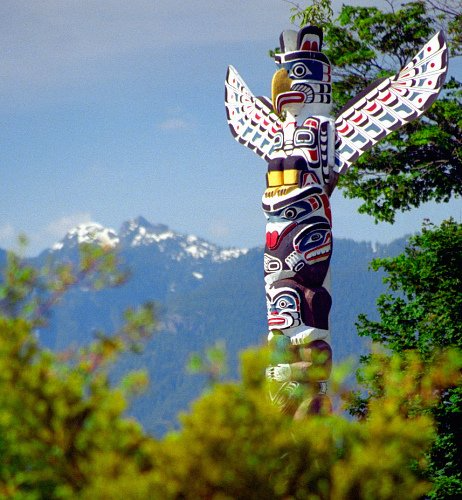
\includegraphics[width=6cm, height=6cm]{stanley-totem-poles.png}
%\caption{原图3}
\end{minipage}
}
\subfigure[结果3]{
\begin{minipage}{0.45\linewidth}
\centering
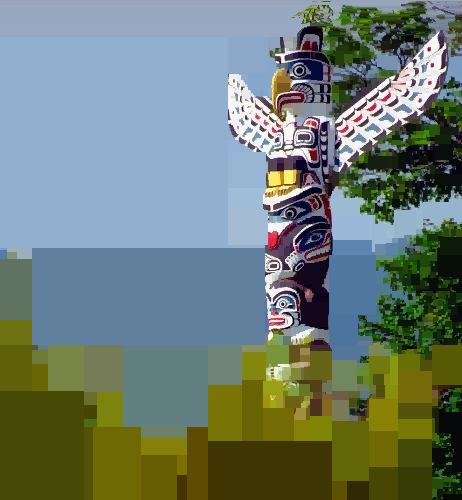
\includegraphics[width=6cm, height=6cm]{prunedstanleytotem.png}
%\caption{结果3}
\label{res3}
\end{minipage}
}

\caption{测试结果}
\label{res123}
\end{figure}

\begin{figure}[H]
\centering
\subfigure[原图4]{
\begin{minipage}{0.45\linewidth}
\centering
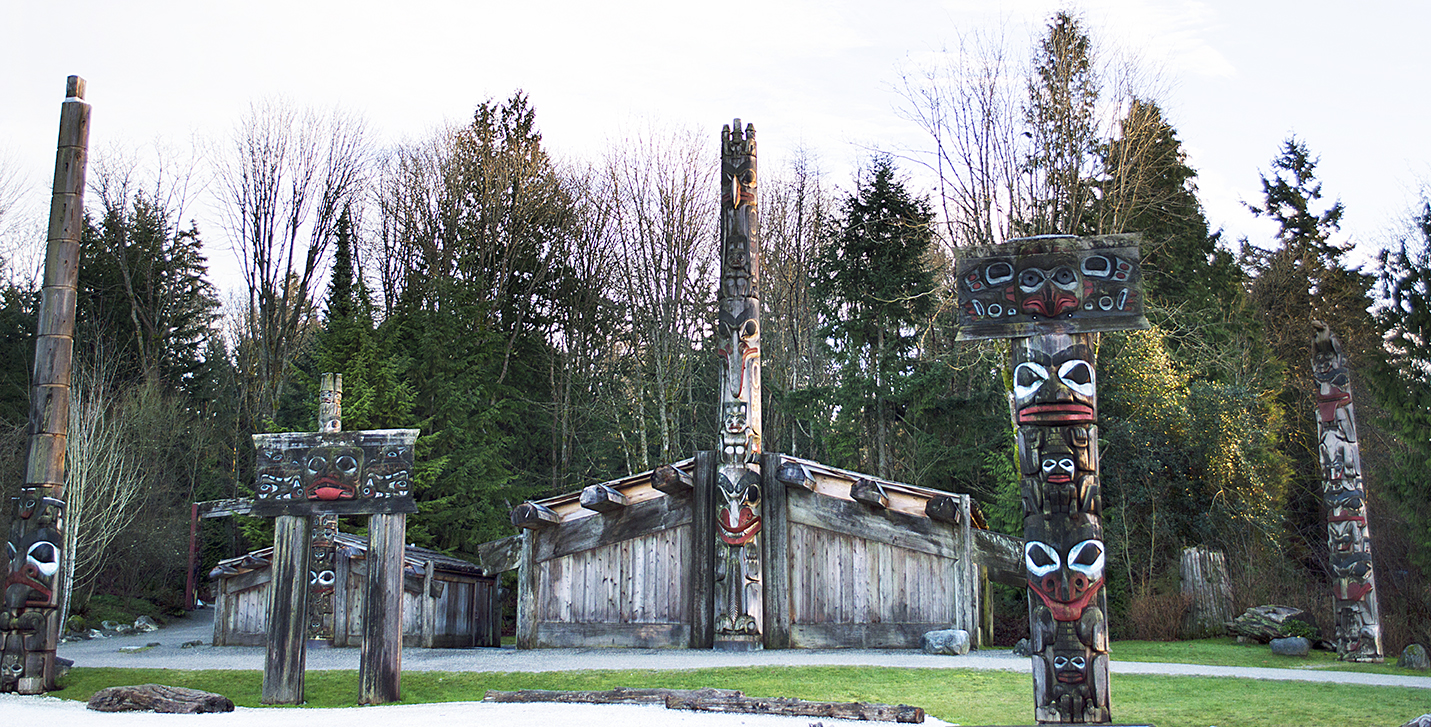
\includegraphics[width=6cm, height=6cm]{ubc-totem-poles.png}
%\caption{原图3}
\end{minipage}
}
\subfigure[结果4]{
\begin{minipage}{0.45\linewidth}
\centering
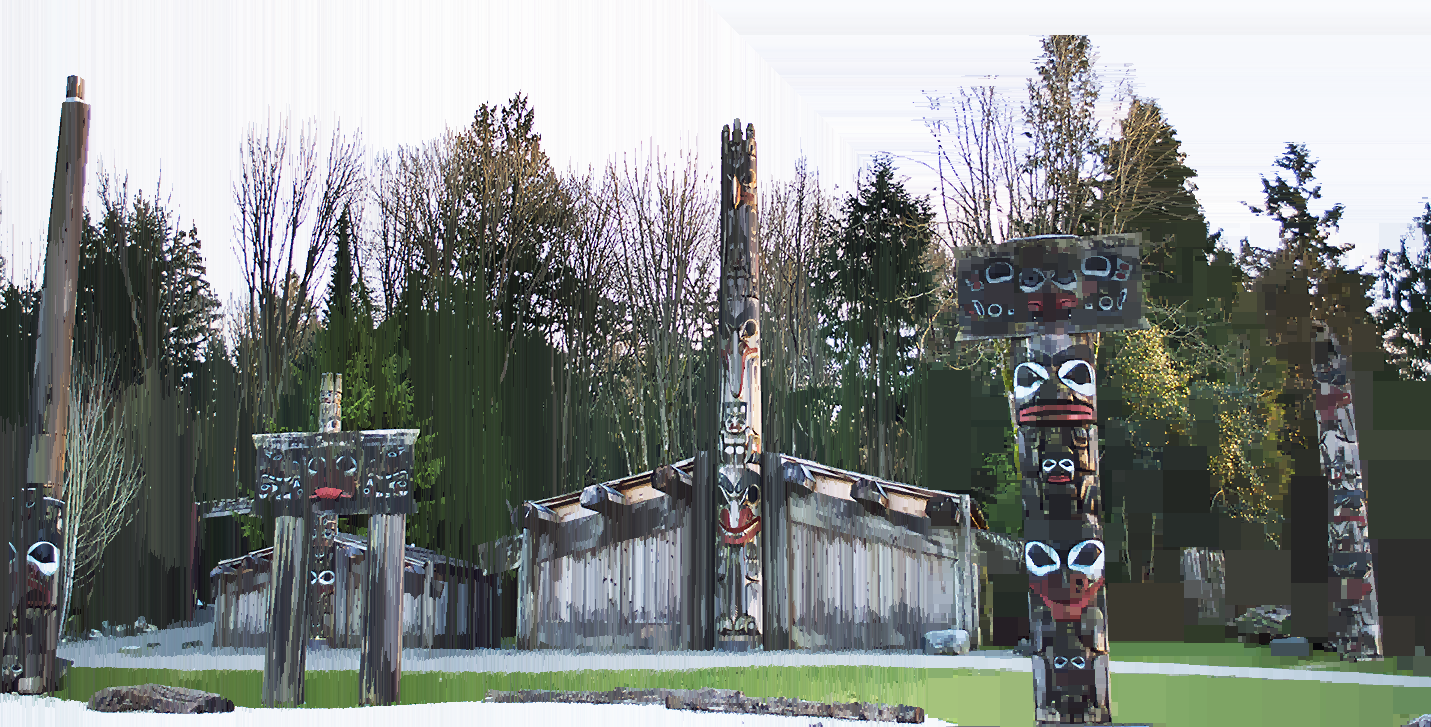
\includegraphics[width=6cm, height=6cm]{prunedubctotem.png}
%\caption{结果3}
\label{res4-4}
\end{minipage}
}

\caption{测试结果}
\label{res4}
\end{figure}




%\begin{figure}[H]
%	\centering 
%	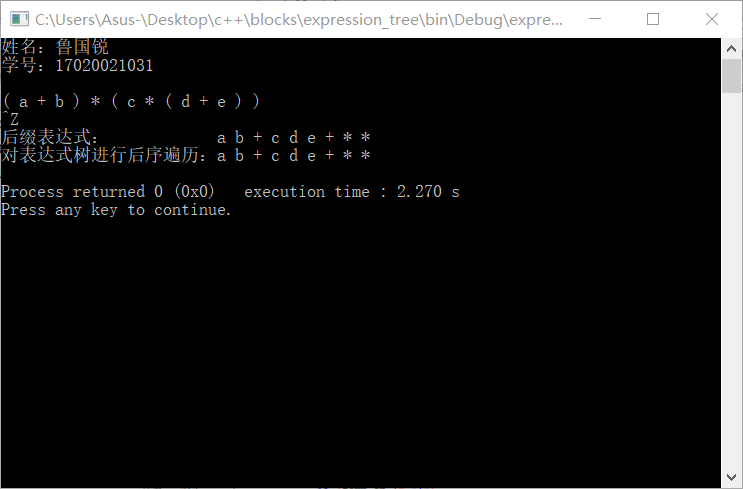
\includegraphics[scale=0.8]{res1.png} 
%	\caption{结果1} 
%	\label{res1}
%\end{figure}



%\begin{figure}[H]
%	\centering 
%	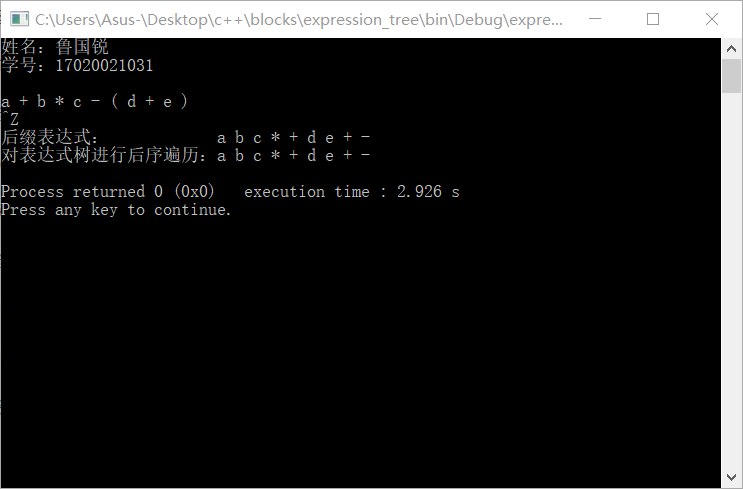
\includegraphics[scale=0.8]{res3.png} 
%	\caption{结果2} 
%	\label{res2}
%\end{figure}

%\begin{figure}[H]
%	\centering 
%	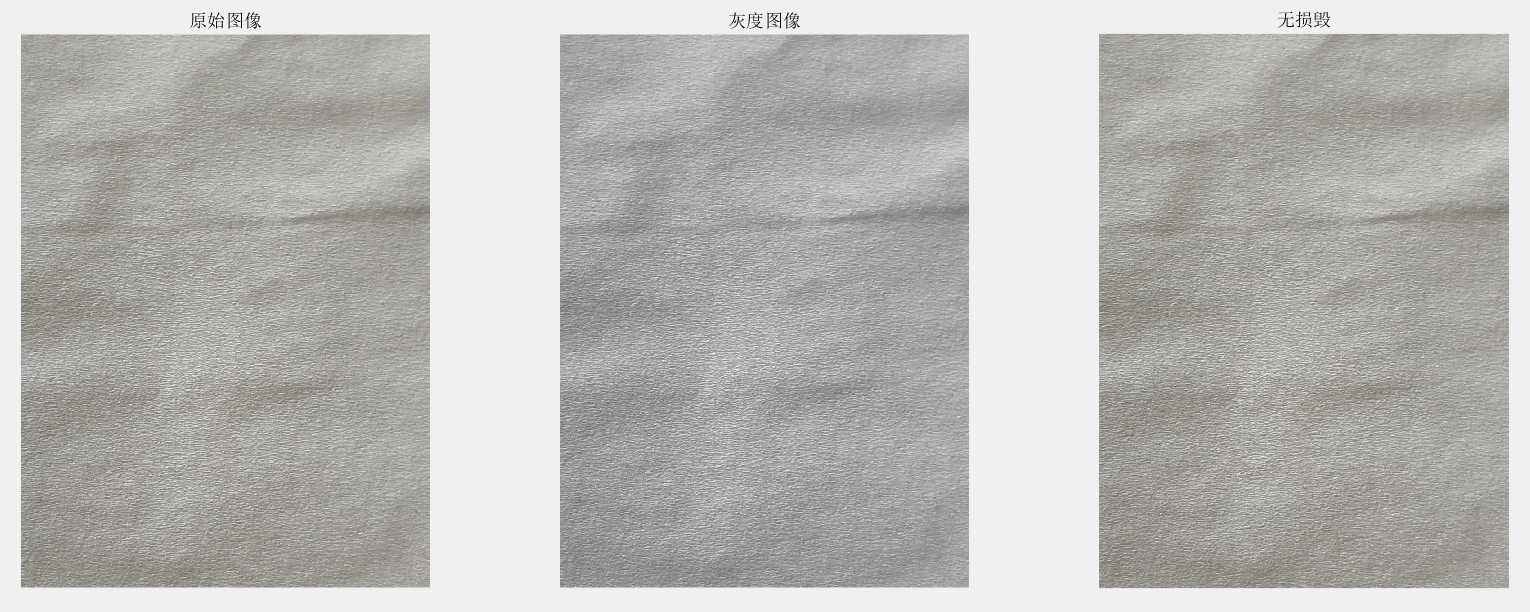
\includegraphics[scale=0.8]{res4.png} 
%	\caption{结果3} 
%	\label{res3}
%\end{figure}

%\begin{figure}[H]
%	\centering 
%	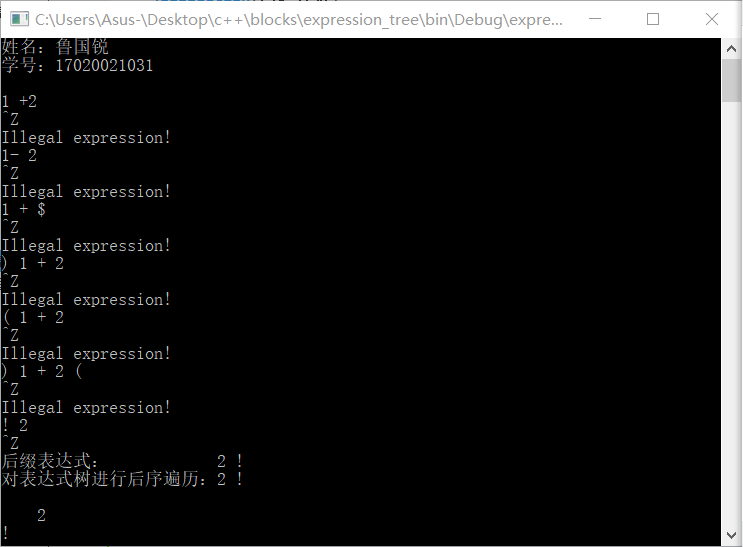
\includegraphics[scale=0.8]{res5.png} 
%	\caption{结果4} 
%	\label{res4}
%\end{figure}



	\subsection{分析}\label{time_of_PrintLots}
	\indent 可以看出,我的结果跟标准结果(报告中未给出)还是有差异的。图\ref{res3}对背景的模糊程度比标准结果要大,而图\ref{res4-4}的模糊程度比标准结果要小。
	
	\indent 这里我所采取的分割方式能保证我们最后一定能把矩形分成一个一个像素。而采取“深度为偶数垂直分割,深度为奇数水平分割”的策略则有可能导致分到一定程度时当前矩形只剩一行(或一列)而深度却刚好是奇数(或偶数),无端增加了考虑的复杂性,而且也没有理论能表明这样分割一定能达到更好的效果,因此我觉得并没有必要局限于$K-D$树的分割方式。
	
	\indent 关于剪枝函数虽然我们用向量作为辅助使得只需要对每一个节点访问一次,但在递归返回的过程中,由于$vector$是在函数内部定义的,在函数结束后变量会被自动销毁,所以我们不能直接返回它的引用。这就导致了在函数返回时采用的是“值传递”,再加上需要合并向量,这就又增加了计算的成本。粗略计算仅对向量进行赋值和合并所需的时间复杂度就已经是一个与$2^{height}\times height$成正比的函数了(每个节点的度数为$0$或$2$),再加上删除和访问,这一块的开销其实相当大。但再仔细考虑一下,$2^{height}$代表的其实是所有叶节点的数量(其实是大于等于叶节点数量),显然$2^{height}\times height$要小于$n^2$,所以总体而言这么做还是值得的。
		

	\section{总结体会}
	\indent 在完成这次作业的过程中,因为代码的不规范出了很多错误。其中印象比较深的是在剪枝时我一开始是把节点作为$vector$的元素,但由于$Node$类中没有写复制构造函数(我花了好长时间才发现这一点),导致程序运行时出了很多奇怪的报错。另外就是在删除一个节点后\textbf{必须把指向该节点的指针置为$NULL$},如果不这样做的话,该指针不为空且指向一片已经被销毁的区域,会导致一些不可预计的后果。
	
	\indent 还有一点就是有时候把变量名取得太相似会使得在打代码的过程中经常会把它们写反。比如在实现$render\_helper$函数时,递归中我用$r$来指代当前节点,结果有几处把$r$跟整棵树的根节点$root$写反了,程序可以正常运行并退出(\textcolor[rgb]{1,0,0}{这是最可怕的的!}),但结果就是不对,导致我在这上面浪费了很多时间,$render\_helper$函数也是我用时最多的一个函数。

\bibliography{ref.bib}
\end{document}